
%(BEGIN_QUESTION)
% Copyright 2006, Tony R. Kuphaldt, released under the Creative Commons Attribution License (v 1.0)
% This means you may do almost anything with this work of mine, so long as you give me proper credit

Calculate values for the following calibration table, for a transmitter measuring liquid level interface (densities = 50 lb/ft$^{3}$ and 70 lb/ft$^{3}$), with a calibration tolerance of $\pm$ 1\% and a 4-20 mA output range:

$$\includegraphics[width=15.5cm]{i00686x01.eps}$$

% No blank lines allowed between lines of an \halign structure!
% I use comments (%) instead, so that TeX doesn't choke.

$$\vbox{\offinterlineskip
\halign{\strut
\vrule \quad\hfil # \ \hfil & 
\vrule \quad\hfil # \ \hfil & 
\vrule \quad\hfil # \ \hfil & 
\vrule \quad\hfil # \ \hfil & 
\vrule \quad\hfil # \ \hfil & 
\vrule \quad\hfil # \ \hfil \vrule \cr
\noalign{\hrule}
%
% First row
Interface & Percent of & $\Delta$ pressure & Output signal & Output signal & Output signal \cr
%
% Another row
level (in) & span (\%) & sensed ("W.C) & ideal (mA) & min. (mA) & max. (mA) \cr
%
\noalign{\hrule}
%
% Another row
  & 0 &  &  &  &  \cr
%
\noalign{\hrule}
%
% Another row
  & 10 &  &  &  &  \cr
%
\noalign{\hrule}
%
% Another row
  & 25 &  &  &  &  \cr
%
\noalign{\hrule}
%
% Another row
  & 50 &  &  &  &  \cr
%
\noalign{\hrule}
%
% Another row
  & 75 &  &  &  &  \cr
%
\noalign{\hrule}
%
% Another row
  & 90 &  &  &  &  \cr
%
\noalign{\hrule}
%
% Another row
  & 100 &  &  &  &  \cr
%
\noalign{\hrule}
} % End of \halign 
}$$ % End of \vbox

\vskip 20pt \vbox{\hrule \hbox{\strut \vrule{} {\bf Suggestions for Socratic discussion} \vrule} \hrule}

\begin{itemize}
\item{} Demonstrate how to {\it estimate} numerical answers for this problem without using a calculator.
\end{itemize}


\underbar{file i00686}
%(END_QUESTION)





%(BEGIN_ANSWER)

\noindent
{\bf Partial answer:}

% No blank lines allowed between lines of an \halign structure!
% I use comments (%) instead, so that TeX doesn't choke.

$$\vbox{\offinterlineskip
\halign{\strut
\vrule \quad\hfil # \ \hfil & 
\vrule \quad\hfil # \ \hfil & 
\vrule \quad\hfil # \ \hfil & 
\vrule \quad\hfil # \ \hfil & 
\vrule \quad\hfil # \ \hfil & 
\vrule \quad\hfil # \ \hfil \vrule \cr
\noalign{\hrule}
%
% First row
Interface & Percent of & $\Delta$ pressure & Output signal & Output signal & Output signal \cr
%
% Another row
level (in) & span (\%) & sensed ("W.C) & ideal (mA) & min. (mA) & max. (mA) \cr
%
\noalign{\hrule}
%
% Another row
0 & 0 & 28.83 &  & 3.84 &  \cr
%
\noalign{\hrule}
%
% Another row
 & 10 &  & 5.6 &  & 5.76 \cr
%
\noalign{\hrule}
%
% Another row
2.75 & 25 & 29.71 &  & 7.84 &  \cr
%
\noalign{\hrule}
%
% Another row
 & 50 &  & 12 &  & 12.16 \cr
%
\noalign{\hrule}
%
% Another row
 & 75 & 31.48 &  & 15.84 &  \cr
%
\noalign{\hrule}
%
% Another row
9.9 & 90 &  & 18.4 &  & 18.56 \cr
%
\noalign{\hrule}
%
% Another row
 & 100 &  & 20 & 19.84 &  \cr
%
\noalign{\hrule}
} % End of \halign 
}$$ % End of \vbox


%(END_ANSWER)





%(BEGIN_NOTES)

LRV = 15 inches of heavy + 15 inches of light = (15 in)(70/62.428) + (15 in)(50/62.428) = 28.83 "WC

\vskip 10pt

URV = 26 inches of heavy + 4 inches of light = (26 in)(70/62.428) + (4 in)(50/62.428) = 32.36 "WC

% No blank lines allowed between lines of an \halign structure!
% I use comments (%) instead, so that TeX doesn't choke.

$$\vbox{\offinterlineskip
\halign{\strut
\vrule \quad\hfil # \ \hfil & 
\vrule \quad\hfil # \ \hfil & 
\vrule \quad\hfil # \ \hfil & 
\vrule \quad\hfil # \ \hfil & 
\vrule \quad\hfil # \ \hfil & 
\vrule \quad\hfil # \ \hfil \vrule \cr
\noalign{\hrule}
%
% First row
Interface & Percent of & $\Delta$ pressure & Output signal & Output signal & Output signal \cr
%
% Another row
level (in) & span (\%) & sensed ("W.C) & ideal (mA) & min. (mA) & max. (mA) \cr
%
\noalign{\hrule}
%
% Another row
0 & 0 & 28.83 & 4 & 3.84 & 4.16 \cr
%
\noalign{\hrule}
%
% Another row
1.1 & 10 & 29.19 & 5.6 & 5.44 & 5.76 \cr
%
\noalign{\hrule}
%
% Another row
2.75 & 25 & 29.71 & 8 & 7.84 & 8.16 \cr
%
\noalign{\hrule}
%
% Another row
5.5 & 50 & 30.60 & 12 & 11.84 & 12.16 \cr
%
\noalign{\hrule}
%
% Another row
8.25 & 75 & 31.48 & 16 & 15.84 & 16.16 \cr
%
\noalign{\hrule}
%
% Another row
9.9 & 90 & 32.00 & 18.4 & 18.24 & 18.56 \cr
%
\noalign{\hrule}
%
% Another row
11 & 100 & 32.36 & 20 & 19.84 & 20.16 \cr
%
\noalign{\hrule}
} % End of \halign 
}$$ % End of \vbox












\vfil \eject

\noindent
{\bf Prep Quiz:}

Suppose a level transmitter with a calibrated range of 40 to 75 inches (4 to 20 mA output) senses a process liquid level of 47 inches.  Calculate the milliamp value this transmitter should output at this level.

\begin{itemize}
\item{} 3.2 mA
\vskip 5pt 
\item{} 5.4 mA
\vskip 5pt 
\item{} 6.2 mA
\vskip 5pt 
\item{} 6.4 mA
\vskip 5pt 
\item{} 7.0 mA
\vskip 5pt 
\item{} 7.2 mA
\end{itemize}






\vfil \eject

\noindent
{\bf Prep Quiz:}

Suppose a level transmitter with a calibrated range of 40 to 75 inches (4 to 20 mA output) senses a process liquid level of 60 inches.  Calculate the milliamp value this transmitter should output at this level.

\begin{itemize}
\item{} 12.0 mA
\vskip 5pt 
\item{} 13.14 mA
\vskip 5pt 
\item{} 8.27 mA
\vskip 5pt 
\item{} 16.8 mA
\vskip 5pt 
\item{} 13.6 mA
\vskip 5pt 
\item{} 9.14 mA
\end{itemize}

%INDEX% Calibration: table, level transmitter (same scenario as i00683)
%INDEX% Measurement, interface level: calibration table (same scenario as i00683)

%(END_NOTES)


